\documentclass[11pt,a4j]{jarticle}%jarticleを使用
\usepackage[dvipdfmx]{graphicx}%画像表示の設定
\usepackage{amsmath}%数式周りの強化
\usepackage[all, warning]{onlyamsmath}%eqnarrayを禁止
\usepackage[top=5truemm,bottom=30truemm,left=20truemm,right=20truemm]{geometry}%ページの余白を調整
\usepackage{cite}%引用を整備
\usepackage{ascmac}%screen環境による箱囲みを利用
\usepackage{url}%urlを成形する
\usepackage{here}
\usepackage{listings,jvlisting} %日本語のコメントアウトをする場合jvlisting(もしくはjlisting)が必要
%ここからソースコードの表示に関する設定
\lstset{
  basicstyle={\ttfamily},
  identifierstyle={\small},
  commentstyle={\smallitshape},
  keywordstyle={\small\bfseries},
  ndkeywordstyle={\small},
  stringstyle={\small\ttfamily},
  frame={tb},
  breaklines=true,
  columns=[l]{fullflexible},
  numbers=left,
  xrightmargin=0zw,
  xleftmargin=3zw,
  numberstyle={\scriptsize},
  stepnumber=1,
  numbersep=1zw,
  lineskip=-0.5ex
}
%ここまで表示に関する設定
\begin{document}
\title{音声情報処理演習まとめ}
\author{学籍番号: 1029332978 氏名: 上野山遼音}
\maketitle
\tableofcontents
\clearpage
\section{演習2}
\begin{figure}[H]
  \centering
  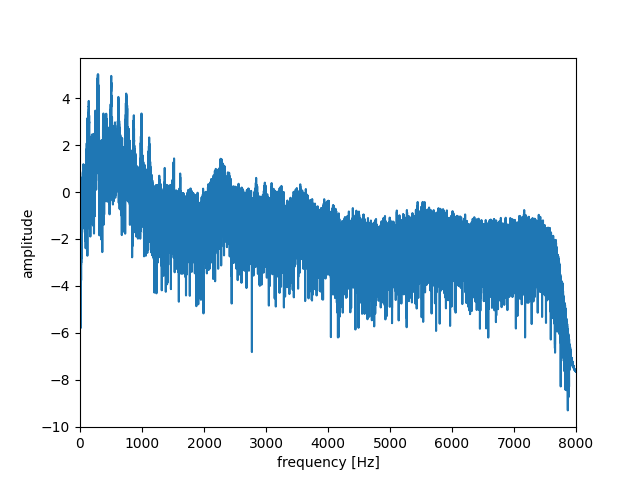
\includegraphics[width=120mm]{img/aiueo-plot-spectrum-whole.png}
  \caption{aiueo.wavの波形とスペクトル}
\end{figure}

\begin{figure}[H]
  \centering
  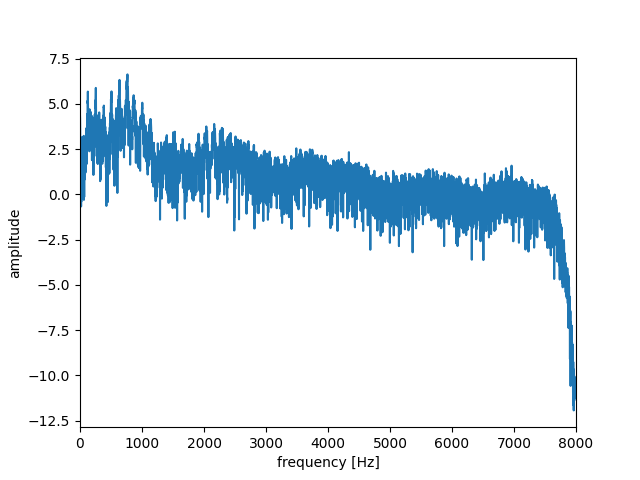
\includegraphics[width=120mm]{img/a-plot-spectrum-whole.png}
  \caption{a.wavの波形とスペクトル}
\end{figure}

\begin{figure}[H]
  \centering
  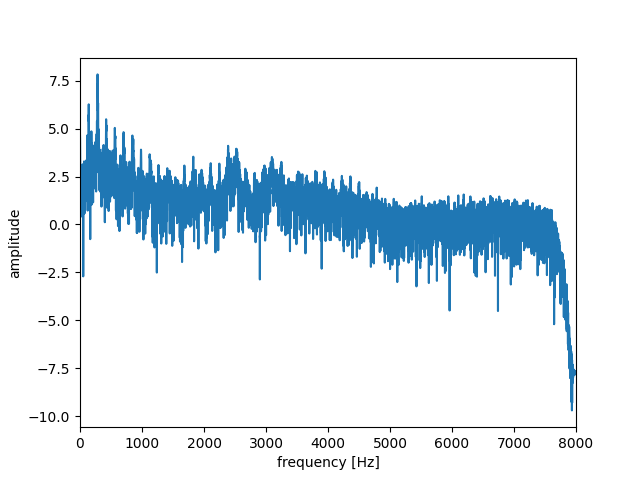
\includegraphics[width=120mm]{img/i-plot-spectrum-whole.png}
  \caption{i.wavの波形とスペクトル}
\end{figure}

\begin{figure}[H]
  \centering
  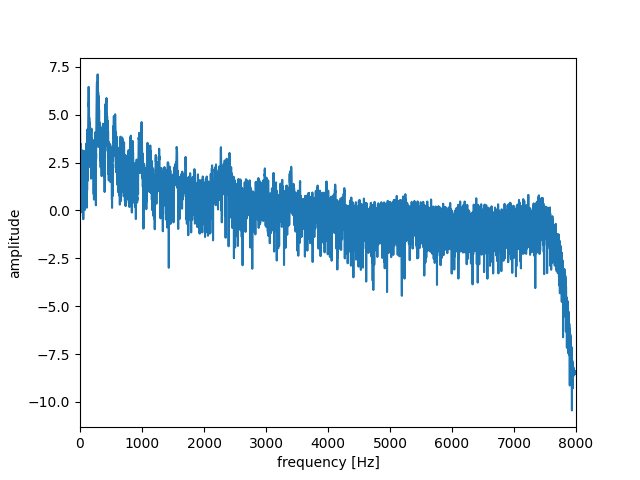
\includegraphics[width=120mm]{img/u-plot-spectrum-whole.png}
  \caption{u.wavの波形とスペクトル}
\end{figure}
\begin{figure}[H]
  \centering
  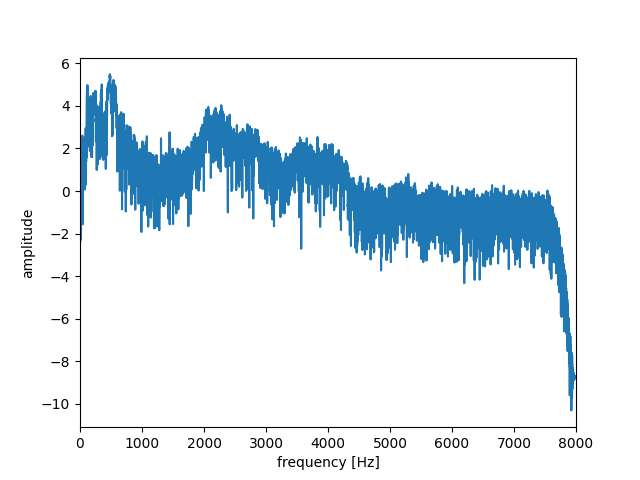
\includegraphics[width=120mm]{img/e-plot-spectrum-whole.png}
  \caption{e.wavの波形とスペクトル}
\end{figure}

\begin{figure}[H]
  \centering
  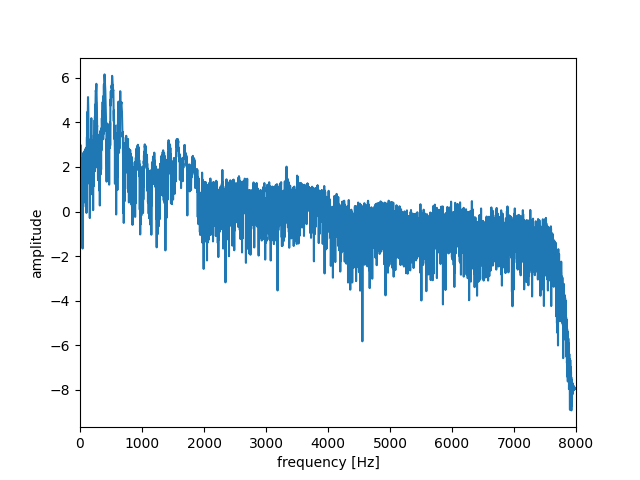
\includegraphics[width=120mm]{img/o-plot-spectrum-whole.png}
  \caption{o.wavの波形とスペクトル}
\end{figure}

\section{演習3}
実数入力に対する1次元離散フーリエ変換を計算するするライブラリ.
高速フーリエ変換(FFT)によって、実数値配列の1次元n点離散フーリエ変換(DFT)を計算する.
入力は実数値配列で、出力は複素数値配列である.
入力には他にも $n$(使用する入力内の変換軸に沿ったポイントの数, optional),axis(変換を行う軸, optional) を指定できる.

※純粋な実数入力に対して DFT を計算すると、出力はエルミート対称($その成分は任意の添字 i, j について (i, j)成分は (j, i)成分の複素共役と等しい.$)になる.
つまり、負の周波数項は対応する正の周波数項の複素共役にすぎない.
したがって負の周波数項は冗長になるのでRFFTでは負の周波数項を計算しない.
その結果、出力の軸の長さは $\lfloor n/2 \rfloor+ 1
$になる.
\section{演習4}
\subsection{バタフライ演算}
\paragraph{DFTについて}
そもそも、DFTでは$N$点の実変数 $f(0),f(1), ... ,f(N-1)$を離散フーリエ変数 $F(0),F(1), ... ,F(N-1)$に変換するために
$N$次正方行列であるDFT行列を掛け合わせているのだった.
この計算では,$O(N^2)$となる.この計算量を軽減するために、高速フーリエ変換(FFT)が考案された. 
\paragraph{FFTの計算量}
上述の通りDFTでは計算量が多いので、バタフライ演算を用いて計算量を減らしている.
\subsection{FFTの実践(手計算)}
input $= (1,0,3,2,4,0,2,0)^T $
\begin{align}
(略)
\end{align}
以下で計算が正しいことを検証する.
\begin{lstlisting}[caption=FFTの実践(numpy篇),label=prog1]
>>> import numpy as np
>>> np.fft.fft([1,0,3,2,4,0,2,0])
array([12.        +0.j        , -4.41421356-2.41421356j,
      0.        +2.j        , -1.58578644-0.41421356j,
      8.        +0.j        , -1.58578644+0.41421356j,
      0.        -2.j        , -4.41421356+2.41421356j])
\end{lstlisting}

\section{演習5}
% \begin{figure}[H]
%   \centering
%   \includegraphics[width=90mm]{img/aiueo-plot-spectrum.png}
%   \caption{「あいうえお」のスペクトログラム}
% \end{figure}
使用した窓関数はハミング窓である.
フレームサイズは512,シフト長は SR($=16000) / 100 = 160$ とした. 
スペクトログラムの縦軸は周波数であり,標本化定理に基づきプロット区間は0から8000Hzまでとした.
また,横軸は時間である.濃淡がx軸上の時間におけるy軸上の周波数の強さを表す。


\section{演習6}
\paragraph{np.fft.rfft と np.fft.fftの違いについて}
どちらも高速フーリエ変換(FFT)を行うものではあるが,np.fft.rfftは実数の入力に対してFFTを行い,
np.fft.fftは複素数の入力に対してFFTを行う.

rfftが存在する理由は、先述のエルミート対称性を利用し、必要な計算数を削減することができる点にある.
\section{演習7}
DFTは(2)式で表される.
\begin{equation}
  F(t) = \sum_{x=0}^{N-1} f(x)e^{-2\pi ixt/N}dx
\end{equation}
ただし,$N=2^M(M\in Z^+)$である.
\begin{lstlisting}[caption=FFT実装,label=prog1]
import numpy as np
import time


def FFT(f: np.ndarray) -> np.ndarray:
    n = len(f)
    w = np.exp(-2j * np.pi / n)
    w_N = w ** np.arange(n//2)
    if n == 1:
        return f[0]
    F_even = FFT(f[::2])
    F_odd = FFT(f[1::2])
    F = np.zeros(n, dtype=np.complex128)
    F[0:n//2] = F_even + w_N * F_odd
    F[n//2:] = F_even - w_N * F_odd

    return F


input_array = np.arange(2**14, dtype=int)
start = time.perf_counter()
FFT(input_array)
end = time.perf_counter()
print(end - start)
start = time.perf_counter()
np.fft.rfft(input_array)
end = time.perf_counter()
print(end - start)

print(np.allclose(FFT(input_array), np.fft.fft(input_array), atol=1e-10))
\end{lstlisting}

\section{演習12}
自己相関はパワースペクトル(振幅スペクトルの 2 乗)の逆フーリエ変換で計算できる. これを証明せよ.
また,このように自己相関を計算することの利点について述べよ.
さらに,この方法を実装し,numpy.correlate() を用いる場合と実行時間を比較せよ

\section*{演習15}
\begin{figure}[H]
  \centering
  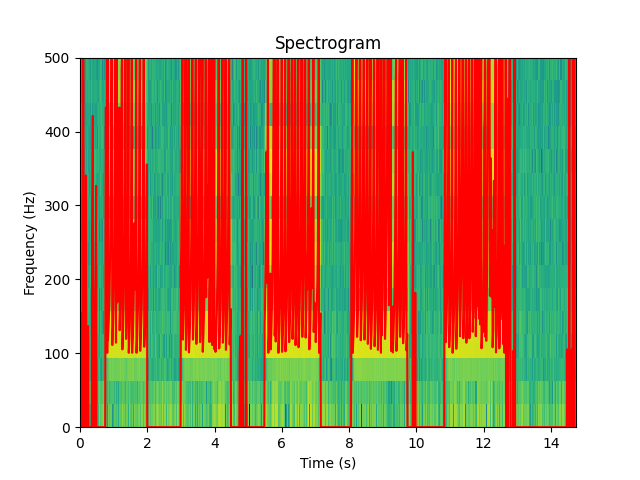
\includegraphics[width=120mm]{img/aiueo2-plot-spectrum-and-fundamental.png}
  \caption{o.wavの波形とスペクトル}
\end{figure}
\section{演習17}

\noindent Q. 共分散行列が対角行列であるときと,そうでないときのそれぞれについて,どのような多次元正規分布を仮定しているのかについて説明せよ.
\\
A. 
\\
$
共分散行列 D = \begin{pmatrix}
  \sigma_{1}^2 & \sigma_{12}^2 & \cdots & \sigma_{1n}^2 \\
  \sigma_{21}^2 & \sigma_{2}^2 & \cdots & \sigma_{2n}^2 \\
  \vdots & \vdots & \ddots & \vdots \\
  \sigma_{n1}^2 & \sigma_{n2}^2 & \cdots & \sigma_{n}^2
\end{pmatrix}
を考える.\\対角行列であれば,\sigma_{ij}^2 = 0 (i \neq j)であるので,任意の共分散が0となり,
確率変数の独立性が仮定されている.
そうでない場合は,共分散が0でないので,独立性は仮定されていない.
$


\section{演習18}
\noindent
Q. 共分散行列が対角行列とみなさない場合について,多次元正規分布の確率密度関数と共分散行列の最尤推定値を示せ.さらに,前述の「あいうえお」の学習と認識について,この共分散行列を仮定し て行い,前述の結果と比較せよ.
\\
A. なんか行列式の微分とかこねくり回せば対角行列と同じ結果になるはず.

\section{演習19}

\end{document}
